\documentclass[tikz,border=10pt]{standalone}
\usepackage[T1]{fontenc}
\usepackage[sfdefault]{FiraSans}
\usepackage{tikz}
\usetikzlibrary{arrows.meta,positioning,calc,decorations.pathreplacing}
\definecolor{navy}{HTML}{003C6C}
\definecolor{navydeep}{HTML}{06294A}
\definecolor{ink}{HTML}{18293B}
\definecolor{muted}{HTML}{5B6B7C}
\definecolor{gold}{HTML}{FDC700}
\definecolor{amber}{HTML}{C98A00}
\definecolor{teal}{HTML}{0E7C9C}
\definecolor{coral}{HTML}{E4572E}
\definecolor{hairline}{HTML}{D9E1E9}
\definecolor{skyfill}{HTML}{E7F0F7}

% STEP is 1..4: elements of step k are full when k==STEP, faded when k<STEP, invisible when k>STEP
% \stepop{k} is replaced by a literal opacity by render_steps.sh (pgfmath cannot evaluate \ifnum in a key)
\begin{document}
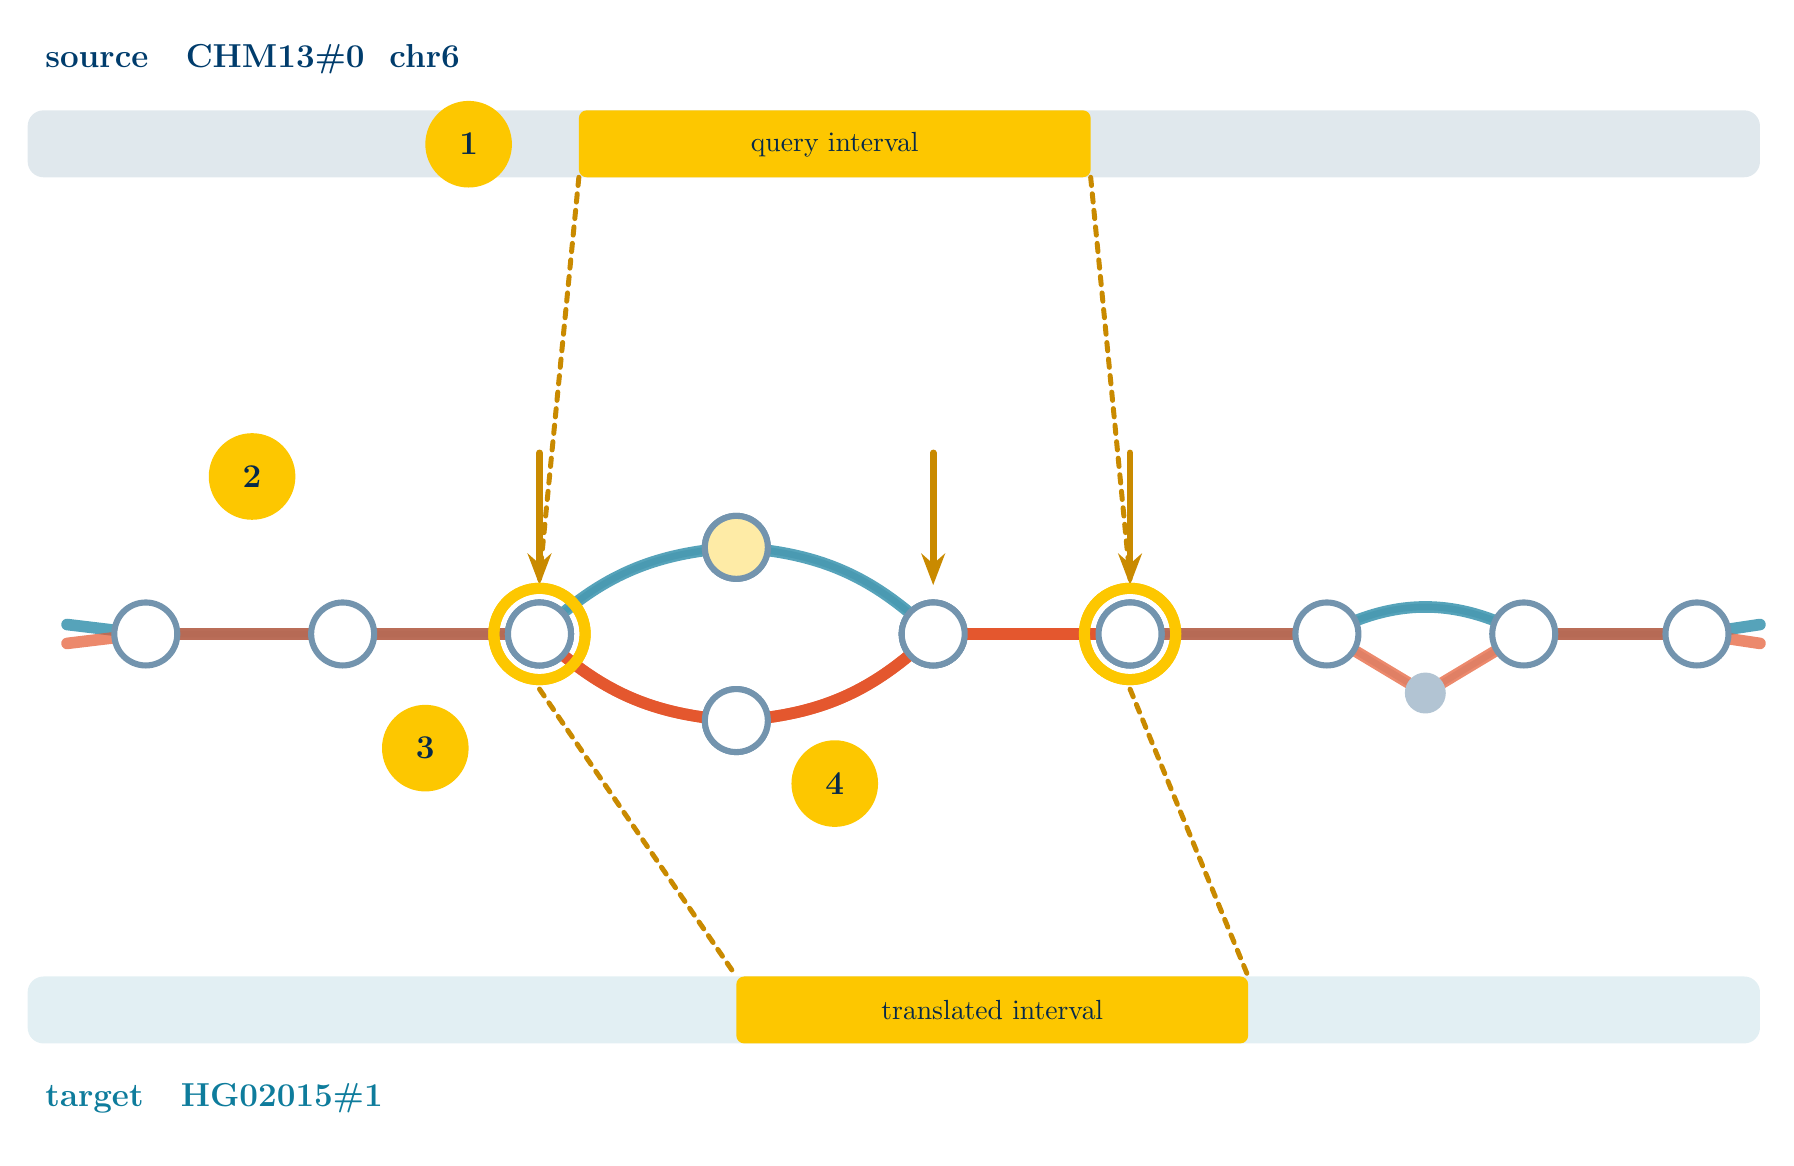
\begin{tikzpicture}[line cap=round]
  % ---- base: source bar with query interval, graph, both paths, target bar ----
  \node[anchor=west, font=\large\bfseries, text=navy] at (0.1,12.5) {source \ \ CHM13\#0 \ chr6};
  \fill[navy!12, rounded corners=2mm] (0,11.0) rectangle (22,11.85);
  \fill[gold, rounded corners=1mm] (7,11.0) rectangle (13.5,11.85);
  \node[font=\normalsize, text=navydeep] at (10.25,11.42) {query interval};
  \coordinate (n1) at (1.5,5.2);  \coordinate (n2) at (4.0,5.2);
  \coordinate (n3) at (6.5,5.2);  \coordinate (bU) at (9.0,6.3);
  \coordinate (bD) at (9.0,4.1);  \coordinate (n4) at (11.5,5.2);
  \coordinate (n5) at (14.0,5.2); \coordinate (n6) at (16.5,5.2);
  \coordinate (n7) at (19.0,5.2); \coordinate (n8) at (21.2,5.2);
  \coordinate (det) at (17.75,4.45);
  \draw[hairline, line width=2.4pt]
    (n1)--(n2)--(n3) (n4)--(n5)--(n6) (n7)--(n8)
    (n3) to[bend left=20] (bU) (bU) to[bend left=20] (n4)
    (n3) to[bend right=20] (bD) (bD) to[bend right=20] (n4)
    (n6) to[bend left=28] (n7) (n6) -- (det) -- (n7);
  \draw[teal, line width=4.2pt, opacity=0.7]
    (0.5,5.32) -- (n1) -- (n2) -- (n3) to[bend left=20] (bU) to[bend left=20] (n4)
    -- (n5) -- (n6) to[bend left=28] (n7) -- (n8) -- (22,5.32);
  \draw[coral, line width=4.2pt, opacity=0.7]
    (0.5,5.08) -- (n1) -- (n2) -- (n3) to[bend right=20] (bD) to[bend right=20] (n4)
    -- (n5) -- (n6) -- (det) -- (n7) -- (n8) -- (22,5.08);
  \foreach \p in {n1,n2,n3,bU,bD,n4,n5,n6,n7,n8}
    {\fill[white] (\p) circle (0.40); \draw[navy!55, line width=2.2pt] (\p) circle (0.40);}
  \fill[navy!30] (det) circle (0.26);
  \fill[teal!12, rounded corners=2mm] (0,0.0) rectangle (22,0.85);
  \node[anchor=west, font=\large\bfseries, text=teal] at (0.1,-0.7) {target \ \ HG02015\#1};

  % ---- step 1: query interval projected onto the source path; its nodes highlighted ----
  \begin{scope}[opacity=\stepop{1}]
    \draw[dashed, amber, line width=1.8pt] (7,11.0) -- (6.5,5.9);
    \draw[dashed, amber, line width=1.8pt] (13.5,11.0) -- (14.0,5.9);
    \foreach \p in {n3,bU,n4,n5} {\fill[gold!35] (\p) circle (0.40); \draw[navy!55, line width=2.2pt] (\p) circle (0.40);}
    \node[fill=gold, circle, minimum size=1.1cm, font=\large\bfseries, text=navydeep] at (5.6,11.42) {1};
  \end{scope}
  % ---- step 2: ask the tag arrays who else is here ----
  \begin{scope}[opacity=\stepop{2}]
    \foreach \p in {n3,n4,n5}
      {\draw[amber, line width=2.4pt, -{Stealth[length=4mm]}] ($(\p)+(0,2.3)$) -- ($(\p)+(0,0.62)$);}
    \node[fill=gold, circle, minimum size=1.1cm, font=\large\bfseries, text=navydeep] at (2.85,7.2) {2};
  \end{scope}
  % ---- step 3: anchors ----
  \begin{scope}[opacity=\stepop{3}]
    \draw[gold, line width=4pt] (n3) circle (0.58);
    \draw[gold, line width=4pt] (n5) circle (0.58);
    \node[fill=gold, circle, minimum size=1.1cm, font=\large\bfseries, text=navydeep] at (5.05,3.75) {3};
  \end{scope}
  % ---- step 4: walk between anchors, emit the translated interval ----
  \begin{scope}[opacity=\stepop{4}]
    \draw[coral, line width=4.2pt] (n3) to[bend right=20] (bD) to[bend right=20] (n4) -- (n5);
    \foreach \p in {n3,bD,n4,n5} {\fill[white] (\p) circle (0.40); \draw[navy!55, line width=2.2pt] (\p) circle (0.40);}
    \draw[gold, line width=4pt] (n3) circle (0.58);
    \draw[gold, line width=4pt] (n5) circle (0.58);
    \fill[gold, rounded corners=1mm] (9,0.0) rectangle (15.5,0.85);
    \node[font=\normalsize, text=navydeep] at (12.25,0.42) {translated interval};
    \draw[dashed, amber, line width=1.8pt] (6.5,4.5) -- (9,0.85);
    \draw[dashed, amber, line width=1.8pt] (14.0,4.5) -- (15.5,0.85);
    \node[fill=gold, circle, minimum size=1.1cm, font=\large\bfseries, text=navydeep] at (10.25,3.3) {4};
  \end{scope}
  % ---- invisible frame so every step has the same bounding box ----
  \path (0,-1.2) rectangle (22,12.9);
\end{tikzpicture}
\end{document}
